\let\negmedspace\undefined
\let\negthickspace\undefined
\documentclass[journal]{IEEEtran}
\usepackage[a5paper, margin=10mm, onecolumn]{geometry}
%\usepackage{lmodern} % Ensure lmodern is loaded for pdflatex
\usepackage{tfrupee} % Include tfrupee package

\setlength{\headheight}{1cm} % Set the height of the header box
\setlength{\headsep}{0mm}     % Set the distance between the header box and the top of the text

\usepackage{gvv-book}
\usepackage{gvv}
\usepackage{cite}
\usepackage{amsmath,amssymb,amsfonts,amsthm}
\usepackage{algorithmic}
\usepackage{graphicx}
\usepackage{textcomp}
\usepackage{xcolor}
\usepackage{txfonts}
\usepackage{listings}
\usepackage{enumitem}
\usepackage{mathtools}
\usepackage{gensymb}
\usepackage{comment}
\usepackage[breaklinks=true]{hyperref}
\usepackage{tkz-euclide} 
\usepackage{listings}
% \usepackage{gvv}                                        
\def\inputGnumericTable{}                                 
\usepackage[latin1]{inputenc}                                
\usepackage{color}                                            
\usepackage{array}                                            
\usepackage{longtable}                                       
\usepackage{calc}                                             
\usepackage{multirow}                                         
\usepackage{hhline}                                           
\usepackage{ifthen}                                           
\usepackage{lscape}
\begin{document}

\bibliographystyle{IEEEtran}
\vspace{3cm}

\title{1.4.28}
\author{EE25BTECH11012-BEERAM MADHURI}
% \maketitle
% \newpage
% \bigskip
{\let\newpage\relax\maketitle}

\renewcommand{\thefigure}{\theenumi}
\renewcommand{\thetable}{\theenumi}
\setlength{\intextsep}{10pt} % Space between text and floats


\numberwithin{equation}{enumi}
\numberwithin{figure}{enumi}
\renewcommand{\thetable}{\theenumi}


\textbf{Question}:\\
Find the position vector of a point $\mathbf{R}$ which divides the line joining two points $\mathbf{P}$ and $\mathbf{Q}$ whose position vectors are $(2\mathbf{a} + \mathbf{b})$ and $(\mathbf{a} - 3\mathbf{b})$ externally in the ratio $1 : 2$. Also, show that $\mathbf{P}$ is the mid point of the line segment $RQ$.
\\
\textbf{Solution: }
\begin{table}[h!]
    \centering
    \begin{tabular}{|c|c|c|c|}
\hline
Angle (\(\alpha\)) & \(\cos(\alpha)\) & Value & Axis \\
\hline
\(90^\circ\) & \(\cos(90^\circ) = 0\) & \(l = 0\) & x-axis \\
\(60^\circ\) & \(\cos(60^\circ) = \frac{1}{2}\) & \(m = \frac{1}{2}\) & y-axis \\
\(30^\circ\) & \(\cos(30^\circ) = \frac{\sqrt{3}}{2}\) & \(n = \frac{\sqrt{3}}{2}\) & z-axis \\
\hline
\end{tabular}
    \caption{Variables used}
    \label{table 1.4.28}
\end{table}

\begin{align*}
 \textbf{R} &= \frac{2(\textbf{P}) - 1(\textbf{Q})}{2 - 1} \\
&= \frac{2(2a+b) - (a-3b)}{1} \\
&= 3a + 5b
\end{align*}
Hence Position vector of $\mathbf{R}$ is 3a + 5b\\
let $\mathbf{P}$ divides $\overline{RQ}$ in k:1 ratio
then 
\begin{align*}
\mathbf{P} &= \frac{k(\textbf{R}) + 1(\textbf{Q})}{k+1} \\
2a+b &= \frac{k(3a+5b) + a-3b}{k+1} \\
(2a+b)(k+1) &= (3k+1)a + (5k-3)b
\end{align*}

\text{Comparing coefficients of } a:
\begin{align*}
2k+2 &= 3k+1 \\
k &= 1
\end{align*}

\text Hence \textbf{P} divides $\overline{RQ}$ in 1:1 ratio, P is midpoint of $\overline{RQ}$.
\begin{figure}[H]
    \centering
    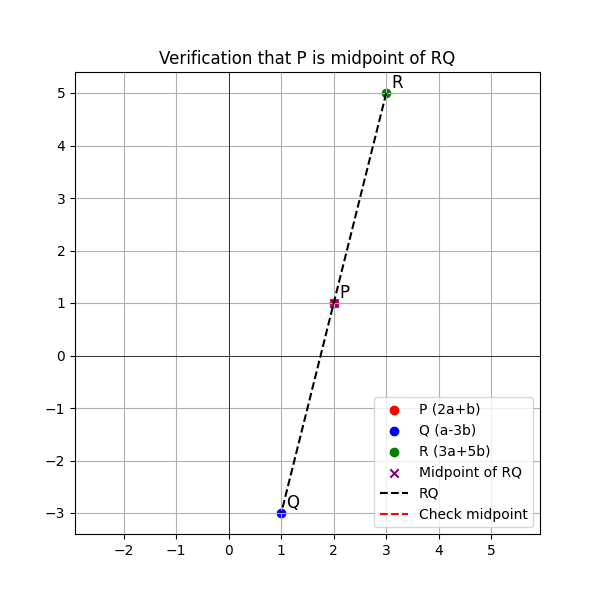
\includegraphics[width=0.75\columnwidth]{figs/graph-1.png}
    \caption{PLOT}
    \label{fig:placeholder}
\end{figure}
\end{document}